\documentclass[11pt, oneside]{article} 
\usepackage{geometry}
\geometry{letterpaper} 
\usepackage{graphicx}
	
\usepackage{amssymb}
\usepackage{amsmath}
\usepackage{parskip}
\usepackage{color}
\usepackage{hyperref}

\graphicspath{{/Users/telliott/Github/precalculus/fig/}}

\title{Polygons}
\date{}

\begin{document}
\maketitle
\Large

Polygons are figures constructed from line segments.  They may have $3$, $4$, $5$ or more sides.  If the sides are all the same, its a \emph{regular} polygon.

\subsection*{quadrilaterals}

Quadrilaterals are four-sided figures.  There are a number of types, some of which are:

$\bullet$ square:  four sides equal, four right angles 

$\bullet$ rectangle:  opposite sides equal, four right angles

$\bullet$ rhombus:  all sides equal, opposite sides parallel

$\bullet$ parallelogram: opposite sides equal and parallel

$\bullet$ trapezoid: two sides parallel

$\bullet$ kite: adjacent sides equal

\subsection*{parallelogram}

Let's look at parallelograms, which can be viewed as two congruent triangles that have been stitched together.

\begin{center} 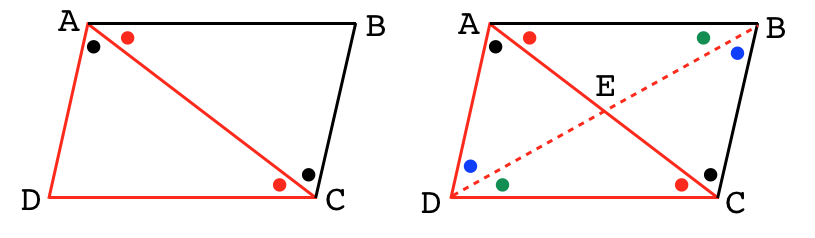
\includegraphics [scale=0.4] {pgram1.png} \end{center}

The definition of a parallelogram is that it is a four-sided figure with opposing sides of equal length and parallel.  Thus, the interior angles theorem gives us the angle equalities shown.  

On the left, we have three angles the same and a shared side, hence $\triangle ABC \cong \triangle ACD$.

Therefore, $AB = DC$ and $AD = BC$.

If we draw the other diagonal and change nothing else, the two triangles are congruent by ASA.  

An important property of parallelograms follows:  the diagonals cross at their midpoints.

\subsection*{rhombus}

If we further constrain all the sides to be equal, then the half triangles like $\triangle ADC$ become isosceles.  

The isosceles triangle theorem says that in a triangle with two sides equal the base angles are equal.  The converse is also true.

By the isosceles triangle theorem, all the angles marked with red dots are equal, and all the blue ones as well.  Because each quarter triangle has a red and a blue, the central angles are all equal.  Therefore, they are all right angles.

\begin{center} 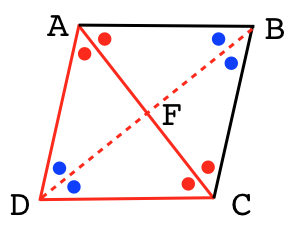
\includegraphics [scale=0.4] {pgram2.png} \end{center}

Now, finally, let us assemble one whole and two have parallelograms starting with the same figure.

\begin{center} 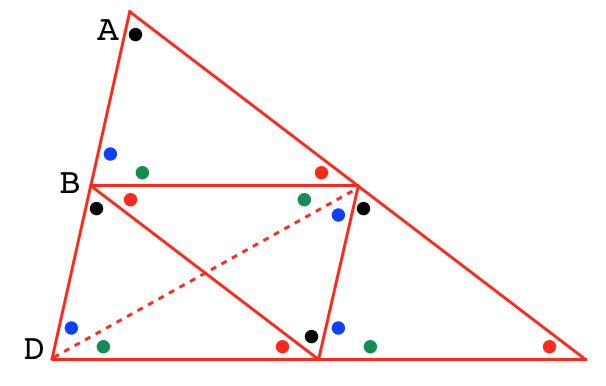
\includegraphics [scale=0.4] {pgram4.png} \end{center}

By the properties of the parallelogram, if the adjacent sides $AB$ and $BD$ are equal, all the angles work out and we get four congruent triangles, so the adjacent sides of the large triangle all have equal segments as well.

\subsection*{pentagons}

Now we explore some properties of a regular pentagon.  The pentagon has five-fold rotational symmetry.  Draw all of the internal chords of the figure and label a few angles.

By rotational symmetry each of the five vertices of the pentagon has the same three components, the central one labeled $s$, and two flanking ones $r$ and $t$.  
\begin{center}
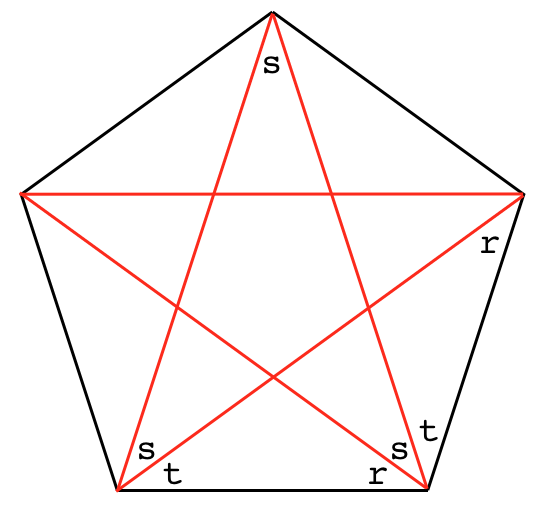
\includegraphics [scale=0.35] {pent1.png}
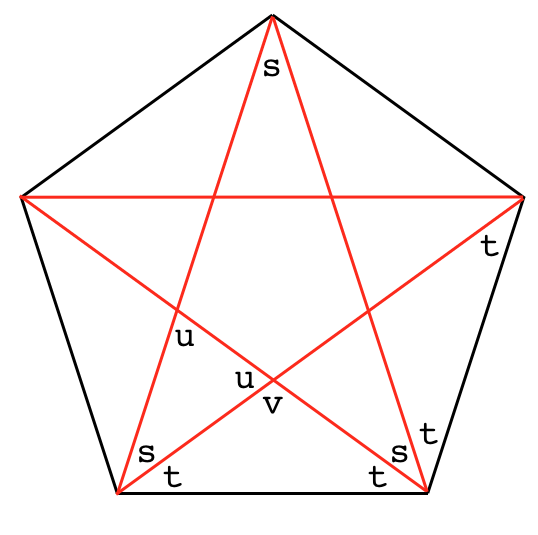
\includegraphics [scale=0.35] {pent2.png}
\end{center}
But $r = t$, by Thales' theorem, using two sides of the pentagon.  Hence we relabel, immediately (right panel).

We compute two triangle sums:
\[ 3s + 2t = 4t + s, \ \ \ \ \ 2s = 2t \]
Hence, $s = t$.  Relabel $t$ as $s$ (left panel, below):
\begin{center}
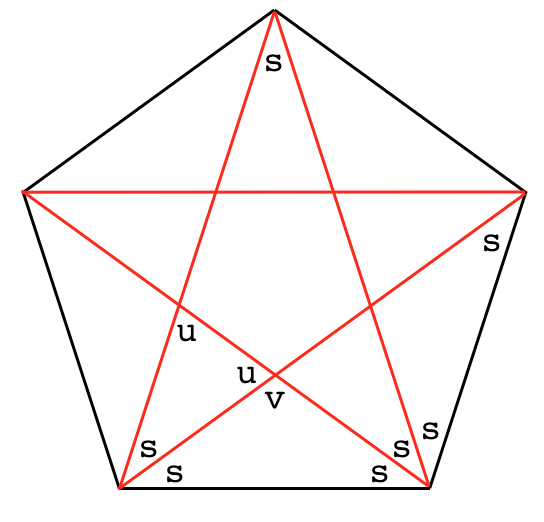
\includegraphics [scale=0.35] {pent3.png}
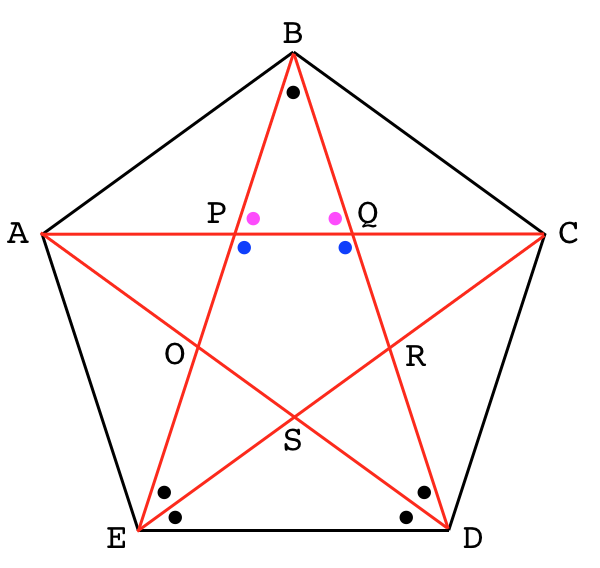
\includegraphics [scale=0.35] {pent4.png}
\end{center}
We observe that $5s = \pi$.
We again compute two triangle sums:
\[ 5s = v + 2s, \ \ \ \ \ v = 3s \]
\[ 5s = 2u + s, \ \ \ \ \ u = 2s \]

Since $v = 3s$, its measure is the same as the vertex angle of the pentagon.  Thus the inner figure is also a regular pentagon.

We do not need the angle labels any more, just the equalities.
\begin{center} 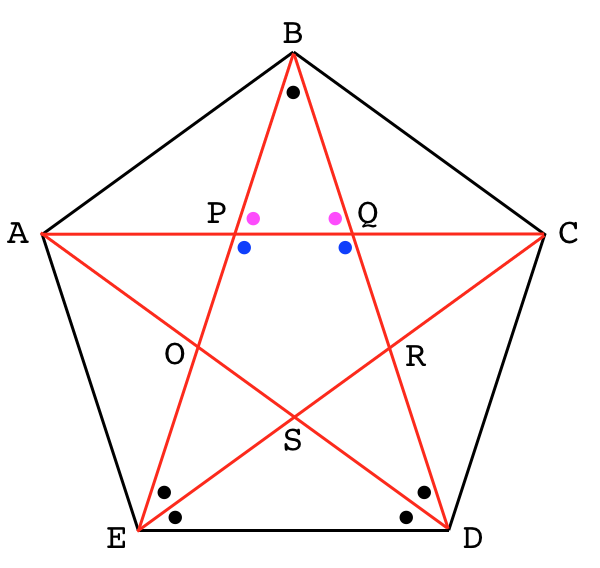
\includegraphics [scale=0.3] {pent4.png} \end{center}

$\triangle BED$ is similar to $\triangle BPQ$.  Hence the side of the inner pentagon is in the same measure to the side of the original pentagon as the ratio of $PQ$ to $AQ$.

Now observe that $AC$ is parallel to $ED$, because they have the equal alternate interior angles of two parallel lines.  (By similar triangles, or simply add the included angles).  Our drawing is filled with regular parallelograms, with four sides equal.

One can draw two types of isosceles triangles using the chords and sides of the pentagon.  One is tall and skinny, the other short and fat.  

The tall, skinny type have base angles equal to $s$.  Here are three examples:
\begin{center} 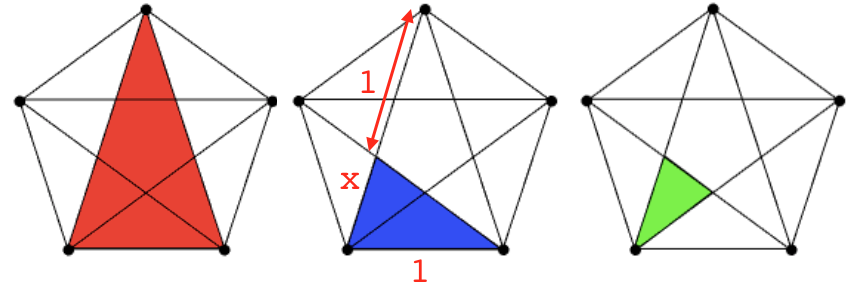
\includegraphics [scale=0.4] {three_triangles_2.png} \end{center}

If we take the side length of the original pentagon to be 1, then all the edges of regular parallelograms in the figure also have side length $1$, so the long side length of the red triangle is $1$ plus some other value, equal to the base of the blue triangle.  Let's call that extra part, $x$.  

We use the fact that red and blue are similar and form the ratio $\phi$ of the long side to the base (red on the left, blue on the right):
\[ \frac{1 + x}{1} = \frac{1}{x} \]
Rearrange:
\[ x^2 + x - 1 = 0 \]
\[ x = \frac{-1 \pm \sqrt{1 + 4}}{2} \]

Of course, $\phi$ is the golden ratio where we have taken the positive branch of the square root:
\[ \phi = 1 + x = \frac{1 + \sqrt{5}}{2} \]

From the similarity of the green triangle, if the side of the inner pentagon is $y$:
\[ \frac{x}{y} = \phi \]
\[ y = \frac{x}{1+x}  \]

\subsection*{hexagon}

A hexagon can be composed of six equilateral triangles.  In an equilateral triangle, the three angles are equal and by the angle sum theorem, their measure is $\pi/3$.  This matches the requirement for a full $6 \cdot \pi/3 = 2 \pi$ angular measure around a point.

\begin{center} 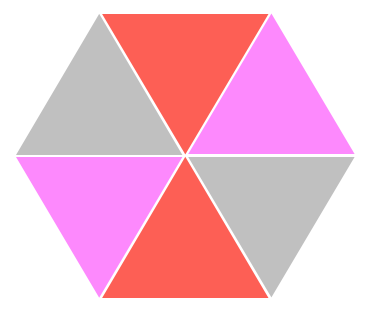
\includegraphics [scale=0.4] {hexagon.png} \end{center}

We simply note numerical verification of the external angle theorem:

\begin{center} 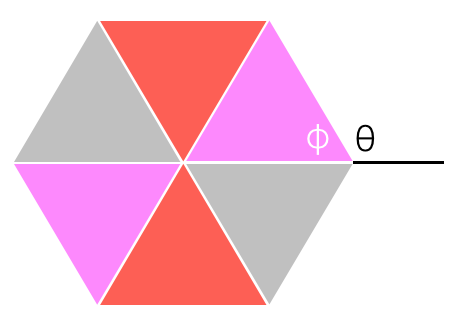
\includegraphics [scale=0.4] {hexagon2.png} \end{center}

\[ \theta = \phi + \phi \]

There is a different theorem, why don't we call it the 

$\bullet$ \ Exterior angle sum theorem

to distinguish the angle from the external angle of a triangle, used above.

Imagine walking all the way around a polygon, to do so we must make $n$ turns.  What is the measure of the angle at each turn, and what is the total angle turned?

It's tricky, because the diagram we have drawn above is not the right one to use.  We need this:

\begin{center} 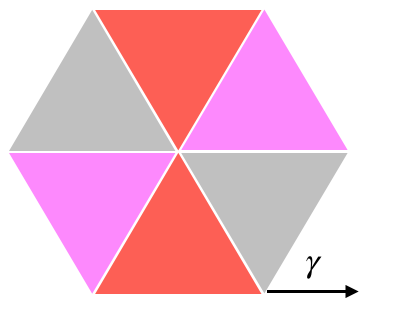
\includegraphics [scale=0.4] {hexagon3.png} \end{center}

Let's recap what we know for the smaller polygons:

$\circ$ \ triangle:  $3 \cdot 2 \pi/3 = 2 \pi$

$\circ$ \ rectangle:  $4 \cdot \pi/2 = 2 \pi$

$\circ$ \ pentagon:  $5 \cdot 2\pi/5 = 2 \pi$

$\circ$ \ hexagon:  $6 \cdot \pi/3 = 2 \pi$

The sum of the external angles is seen to be $2 \pi$, which makes sense.  We simply turn through $2 \pi = 360$ degrees total.  Therefore each angle is $2 \pi / n$.


\end{document}